\chapter{Metodología}

\section{Consideraciones generales}

Para realizar el análisis por elemento finito se han tomado sólo los elementos formadores que 
tienen influencia directa o contacto sobre el formado del tubo, quitando todos los elementos 
del troquel adicionales. Además, los formadores se han considerado como elementos rígidos, 
para simplificar y agilizar el análisis numérico, al permanecer sus características geométricas 
invariables, siendo solamente el blank un sólido deformable.

\section{Geometrías y partes}

En ANSYS/LS-DYNA el concepto de parte es fundamental e incluye dentro de este a todos aquellos 
elementos que comparten el tipo de material, tipo de elemento y sección. Así, es preferible que 
cada componente o pieza se defina como una parte, aun cuando las propiedades elasto-plásticas 
sean iguales. Por ello, para cada una de los componentes del troquel se definió un material 
distinto (aunque con las mismas propiedades).

\begin{center}
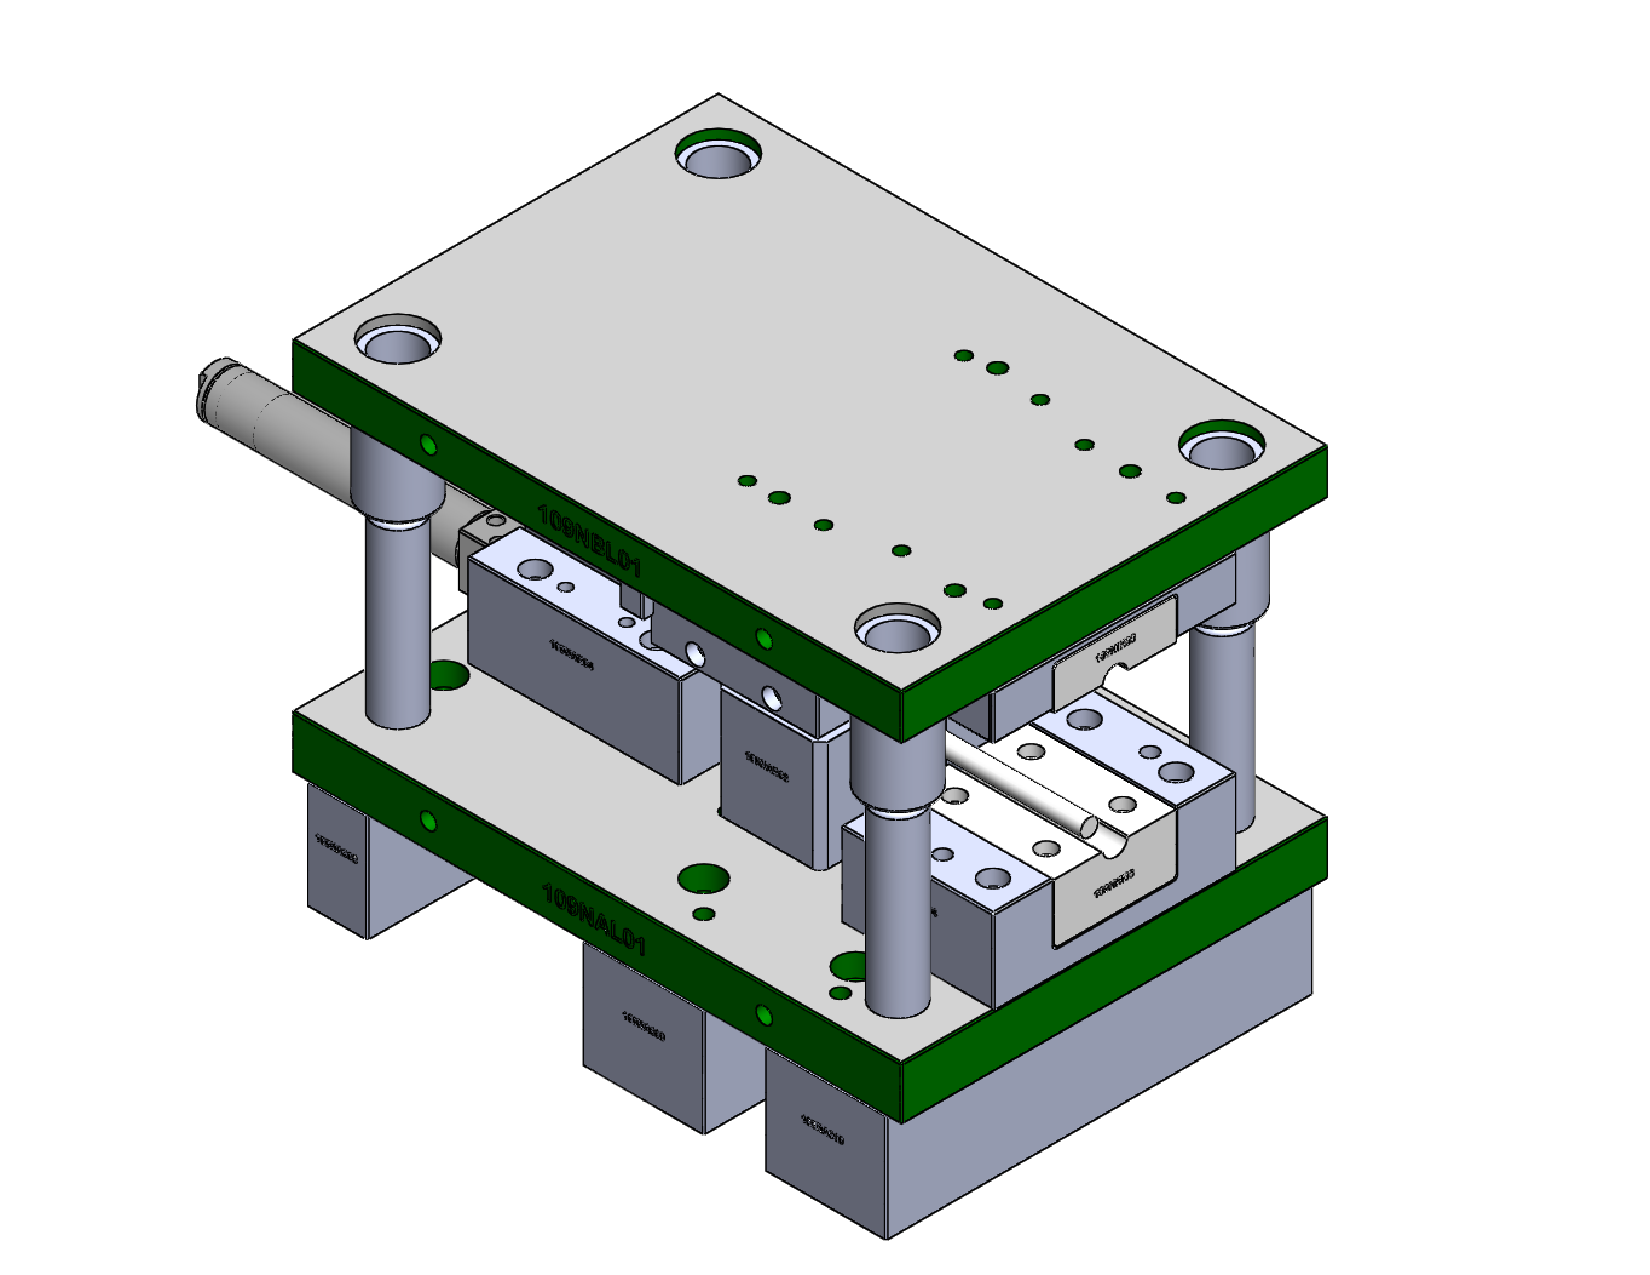
\includegraphics[scale=0.55]{src/ch3/troquel}
\captionof{figure}{Vista completa del troquel}
\label{fig:all_tool}
\end{center}

\section{Modelo constitutivo}

Se utilizó un modelo de tipo \textit{Piecewise Linear Plasticity}, el cual es un modelo multilineal 
que permite utilizar una curva esfuerzo-deformación y la dependencia de la tasa de deformación 
como datos de entrada para definir el comportamiento plástico del material. Para cuantificar 
la tasa de deformación este modelo utiliza la relación de Cowper-Symonds \\

En los componentes del troquel se utilizó un modelo rígido, para el cual sólo es necesario 
especificar las propiedades elásticas. Los componentes rígidos, normalmente, permiten la 
aplicación de condiciones de desplazamiento utilizando el identificador de la parte, además 
de que se pueden asignar propiedades de inercia o velocidades iniciales. En este caso, no se 
especificaron propiedades adicionales, lo cual implica que ANSYS/LS-DYNA calcule automáticamente 
las propiedades inerciales basadas en el modelo de elemento finito.

\section{Mallado}


\begin{center}
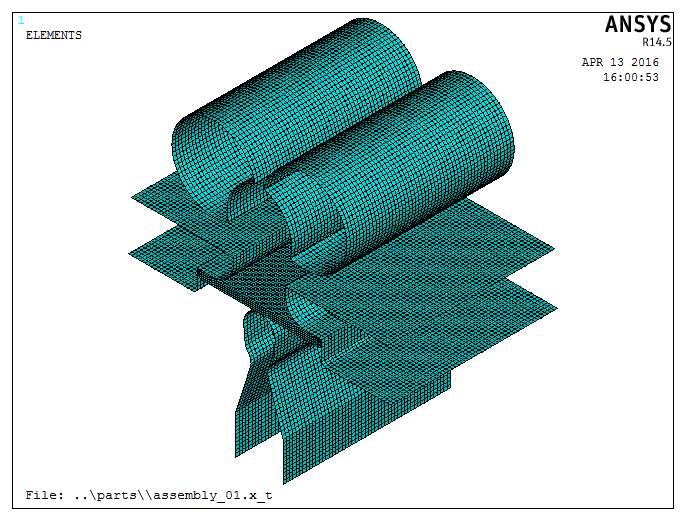
\includegraphics[scale=0.6]{src/ch3/mesh_assembly_01.png}
\captionof{figure}{Mallado del ensamble, primer paso}
\label{fig:mesh_assembly01}
\end{center}

\begin{center}
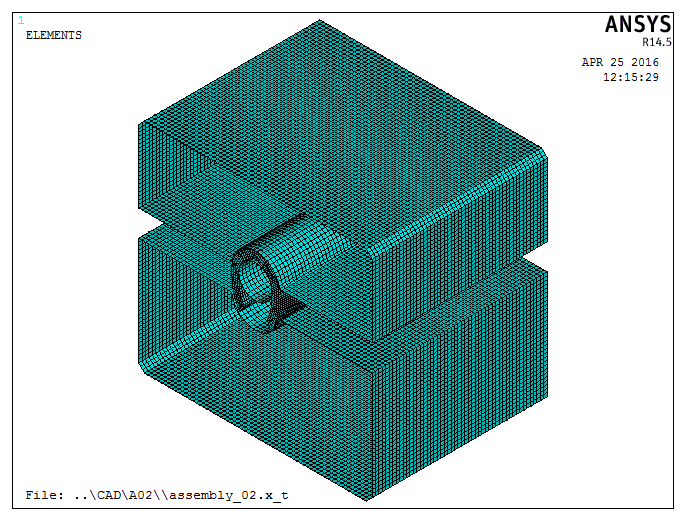
\includegraphics[scale=0.6]{src/ch3/mesh_assembly_02.png}
\captionof{figure}{Mallado del ensamble, segundo paso}
\label{fig:mesh_assembly02}
\end{center}

\section{Condiciones de frontera}

\begin{center}
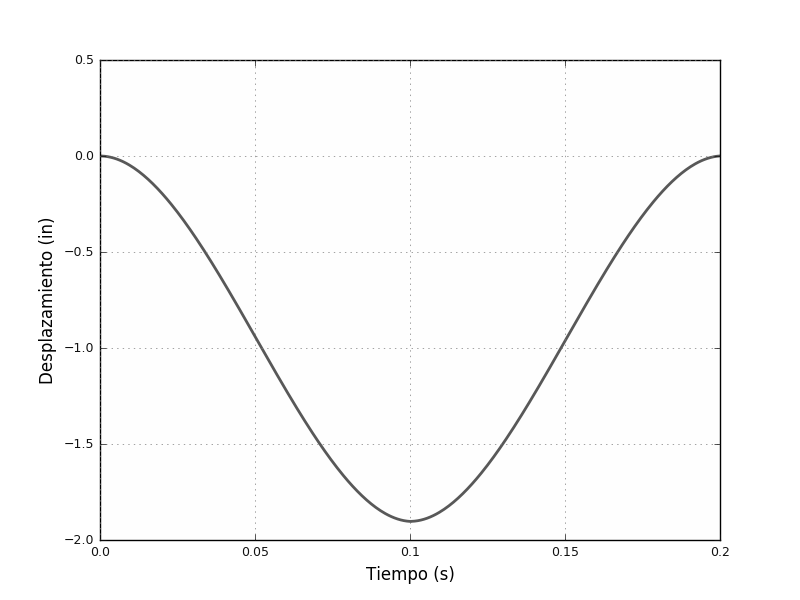
\includegraphics[scale=0.6]{src/ch3/smooth_displacement.png}
\captionof{figure}{Vector de tiempo desplazamiento}
\label{fig:smooth_displacement}
\end{center}




